\documentclass{beamer}
\usepackage{graphicx}
\usepackage{xcolor}
\usepackage{listings}
%Information to be included in the title page:
\title{Lenstra Elliptic Curve Factorization}
\author{Anonymous}
\institute{MATH 317}
\date{2021}

\definecolor{codegray}{rgb}{0.5,0.5,0.5}
\definecolor{backcolour}{rgb}{0.984, 0.945, 0.780}
\definecolor{keyword}{rgb}{0.267,0.478,0.349}
\definecolor{code}{rgb}{0.235,0.220,0.212}

\lstdefinestyle{mystyle}{
    backgroundcolor=\color{backcolour},
    keywordstyle=\color{keyword},
    numberstyle=\tiny\color{codegray},
    basicstyle=\ttfamily\footnotesize\color{code},
    breakatwhitespace=false,
    breaklines=true,
    captionpos=b,
    keepspaces=true,
    numbers=left,
    numbersep=5pt,
    showspaces=false,
    showstringspaces=false,
}

\lstset{style=mystyle}

\begin{document}

\frame{\titlepage}


\begin{frame}
\frametitle{Background 1-2 min}

\center
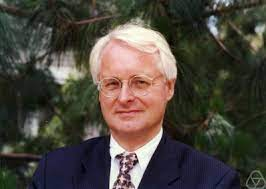
\includegraphics[scale = .5]{lenstra.jpeg}

\begin{itemize}
\item Hendrik Lenstra Jr. recieved his doctorate from the University of Amsterdam in 1977.

\item Discovered Elliptic Curve Factorization (ECM) in 1987.

\item ECM is third-fastest known factoring algorithm and the best algorithm for finding divisors not exceeding 50-60 digits.

\item The largest factor found using ECM has 83 digits.
\end{itemize}
\end{frame}

\begin{frame}
\frametitle{Why Pollard $p-1$ Works.}
$\textbf{Lemma 2.2.5}$ Suppose that $m$, $n \in \mathbb{N}$ and gcd$(a,n) = 1$. Then the map
$$
    \psi : \left( \mathbb{Z}/mn\mathbb{Z} \right)^* \rightarrow \left( \mathbb{Z}/m\mathbb{Z} \right)^* \times \left( \mathbb{Z}/n\mathbb{Z} \right)^*
$$
defined by
$$
    \psi(c) = (c \pmod{m}, c\pmod{n})
$$
is a bijection.

\end{frame}


\begin{frame}
\frametitle{Example by hand 2 mins}

\begin{itemize}
\item Let $B_i = \text{lcm}(1,\ldots, i)$.
\end{itemize}

\center
\begin{tabular}{c|c|c}

$B_i$ & $2^i \pmod{1763} $& $(2^i \pmod{41}, 2^i \pmod{43})$ \\
\hline
1 & 2 & (2,  2) \\
2 & 4 &  (4, 4 )\\
6 &570 & (37, 11) \\
60 & 575 & (1, 16)
\end{tabular}

\begin{itemize}
\item We compute $gcd(574, 1763) = 41$
\end{itemize}
\end{frame}

\begin{frame}
\frametitle{Preliminaries 2 mins}
\begin{itemize}
\item Let $E$ be an elliptic curve over $\mathbb{Z}/N\mathbb{Z}$ of the form
$$
	y^2 = x^3 + ax + 1
$$
such that $4a^3 + 27 \in \left(\mathbb{Z}/N\mathbb{Z}\right)^*$. This forces non singularity and ensures $P = (0,1)$ is on the curve.

\item Definition 6.3.1 (Power Smooth). Let $B$ be a positive integer. If $n$ is a positive integer with prime factorization
$$
    n = \prod p_i^{e_i},
$$
then $n$ is $B$-power smooth if $p_i^{e_i} \leq B$ for all $i$.

\item Example $30 = 2\cdot 3\cdot 5$ is $B$ power smooth for $B \geq 5$, but $150 = 2\cdot 3 \cdot 5^2$ is not $5$-power smooth.
\end{itemize}
\end{frame}

\begin{frame}
\frametitle{Motivation 1-2 mins}
% Explain why p-1 not being B power smooth for a fixed B is a problem
\begin{itemize}
\item Fix $B \in \mathbb{N}$. Let $p \in \mathbb{N}$ such that $p-1$ is not $B$- power smooth.

\item Recall, in Pollard $p-1$, this would be equivalent to not having $p-1 \not \vert m = \text{lcm}(1,2, \ldots, B)$; i.e. $a^m \not \equiv 1 \pmod{p}$.

\item On the interval $[10^{15}, 10^{15} + 10000]$ 15 percent of the primes $p$ are such that $p-1$ is not $10^{6}$-power smooth.

\item The idea of ECM is to replace modular exponentiation on $\left(\mathbb{Z}/N\mathbb{Z}\right)^*$ by repeated addition of points on $E\left(\left(\mathbb{Z}/N\mathbb{Z}\right)^*\right)$

\item Recall, by the Hasse-Weil bound we can reduce the size of our group by $2\cdot \sqrt{p}$.
\end{itemize}
\end{frame}

\begin{frame}
\frametitle{Elliptic Curve Factorization 2 mins}
Algorithm 6.3.10 (Elliptic Curve Factorization Method). Let $N$ and $B$ be positive integers.
\begin{itemize}
\item[1.] Compute $m =$ lcm$(1,2,\ldots, B)$.
\item[2.] Choose $a \in \mathbb{Z}/N\mathbb{Z}$ such that $4a^3 + 27 \in \left(\mathbb{Z}/N\mathbb{Z}\right)^*$. This forces $P = (0,1)$ to be a point on $y^2 = x^3 + ax +1$ over $\mathbb{Z}/N\mathbb{Z}$.
\item[3.] Try to compute $mP$. If at somepoint we cannot compute a sum of points, then some denominator $g$ is not coprime to $N$, then $gcd(g,N)$ is a nontrivial divisor of $N$.
\end{itemize}
\end{frame}

\begin{frame}
\frametitle{Analogy to Pollard p-1 1 min}
\begin{table}[h!]
  \begin{center}
    \caption{Let $E$ be an elliptic curve, and $m = lcm(1,2,\ldots,B)$ for some $B$}
    \label{tab:table1}
    \begin{tabular}{|c|c|} % <-- Alignments: 1st column left, 2nd middle and 3rd right, with vertical lines in between
      \textbf{Pollard $p-1$} & \textbf{ECM} \\
      \hline
      $\mathbb{Z}/N\mathbb{Z}$ & $E\left( \mathbb{Z}/N\mathbb{Z} \right)$\\ &\\
      $g \in (\mathbb{Z}/N\mathbb{Z})^*$ & $(0,1)$ \\ & \\
      $g^m \equiv 1 \pmod{N}$ & $mP \notin E\left( \mathbb{Z}/N\mathbb{Z} \right)$ \\ &\\
      $gcd(g^m-1, N)$ & $gcd(m,N)$
    \end{tabular}
  \end{center}
\end{table}

\begin{itemize}
\item If Pollard $p-1$ fails, we have no choice but to increase $B$.
\item However, ECM has a second option. We can choose another random elliptic curve.
\end{itemize}
\end{frame}


\begin{frame}
\frametitle{Why ECM "Works"}
We can consider an analogous mapping
$$
	"g: E(\mathbb{Z}/N\mathbb{Z}) \rightarrow \prod E(\mathbb{Z}/p\mathbb{Z})"
$$
where $p$ are prime divisors of $N$.

\begin{itemize}
\item Note the quotations. There is a subtly in the difference between $E(\mathbb{Z}/N\mathbb{Z})$ and $\mathbb{Z}/N\mathbb{Z}$.
\item  Let $P = (0:1:1) \in E(\mathbb{Z}/1763\mathbb{Z}$ $P_1 = (0:1:1) \in E(\mathbb{Z}/41\mathbb{Z})$ and $P_2 = (0:1:1) \in E(\mathbb{Z}/43\mathbb{Z})$
\end{itemize}
\end{frame}

\begin{frame}
\frametitle{Example}
\begin{tabular}{l|l|l|l}
i & $i*P_1$ & $i*P_2$ & $i*P$ \\
\hline
0 & (0 : 1 : 1) & (0 : 1 : 1) & (0 : 1 : 1)\\
1 & (1 : 39 : 1)& (1 : 41 : 1) & (1 : 1761 : 1) \\
2 & (8 : 23 : 1)& (8 : 23 : 1) & (8 : 23 : 1) \\
3 &(38 : 38 : 1)& (13 : 17 : 1) & (1432 : 1350 : 1) \\
4 &(23 : 23 : 1) & (2 : 23 : 1) & (1335 : 23 : 1) \\
5 &(20 : 28 : 1) & (33 : 23 : 1) & (635 : 1012 : 1) \\
6 &(26 : 9 : 1) & (20 : 0 : 1) & (149 : 1075 : 1) \\
7& (10 : 18 : 1) &(33 : 20 : 1) & (420 : 1740 : 1) \\
8& (22 : 19 : 1) &(2 : 20 : 1) & (432 : 880 : 1)\\
9 &(40 : 11 : 1) &(13 : 26 : 1) & (1475 : 585 : 1)\\
10 &(19 : 25 : 1) &(8 : 20 : 1) & (1126 : 1009 : 1)\\
11& (32 : 19 : 1)& (1 : 2 : 1) & (1549 : 1249 : 1) \\
12& (13 : 25 : 1)& (0 : 42 : 1) & gcd(denom,$N$) = 43 \\
13 &(12 : 21 : 1) &(0 : 1 : 0) &
\end{tabular}
\end{frame}

\begin{frame}
\frametitle{Implementation}

\begin{itemize}
    \item Generate a random elliptic curve $E \pmod{N}$ and let $P = (0,1)$.
    \item Compute $m = lcm(1,2,...,B)$.
    \item Compute $mP$ (don't be naive!).
    \item If the calculation fails, you have found a non-trivial factor of $N$.
    \item Otherwise, just generate a new Elliptic curve and try again.
    % The calculation can sped up with $\ldots 3 \cdot (2 \cdot P)$.
    % \item Further optimization is possible using the Sieve of Eratosthenes (\texttt{prime\_range()}).
\end{itemize}

\end{frame}

\begin{frame}
\frametitle{Computing lcm(1,2,...,B)}

Recall,

\[ lcm(1,2,...B) = \prod_{p \in P} p^r \]

where $r = \text{max} \{ r \in \mathbb{Z} \mid p^r \leq B \}$.

\begin{align*}
    p^r &\leq B \\
    r\log(p) &\leq \log(B) \\
    r &\leq \log_p(B) \\
    r &= \lfloor \log_p(B) \rfloor \\
\end{align*}

\end{frame}

\begin{frame}

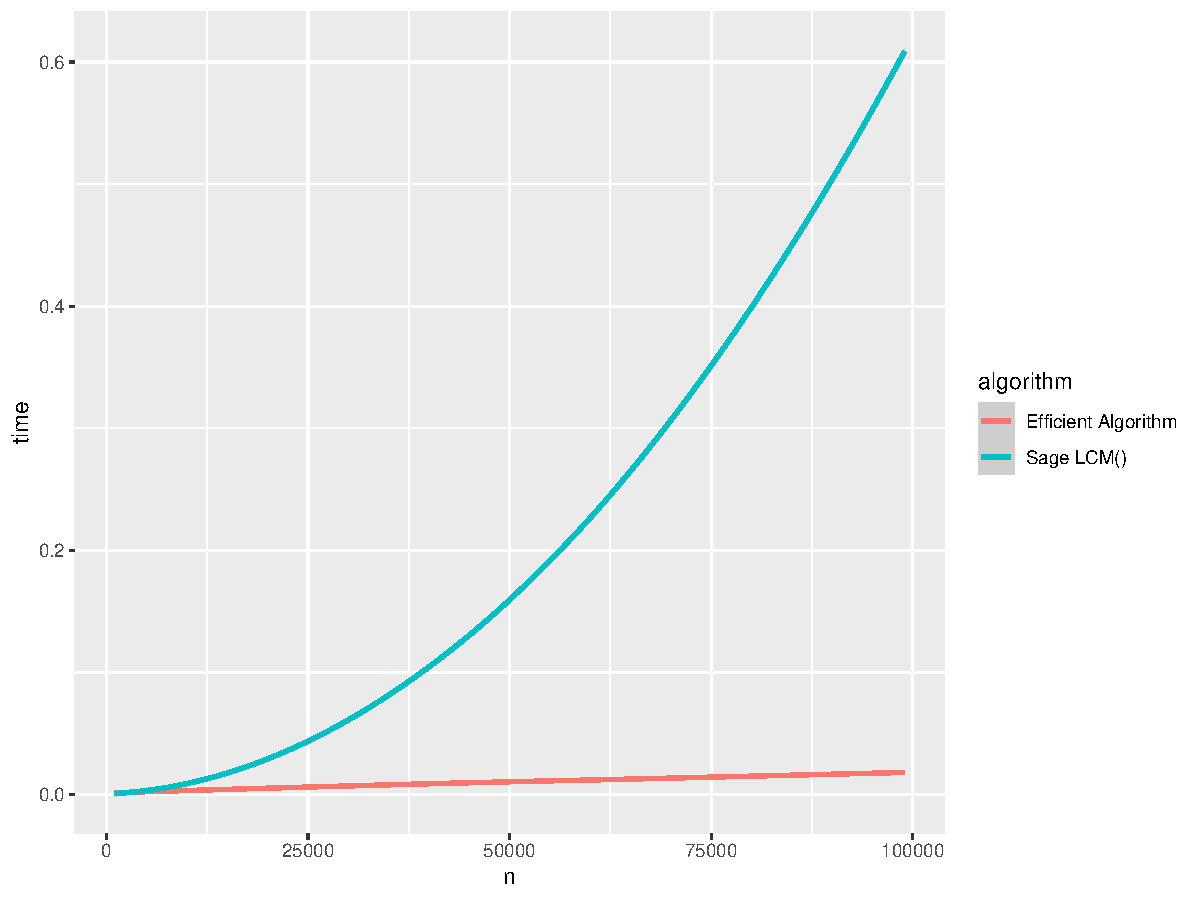
\includegraphics[width=\textwidth]{graphs/lcm_comparison.pdf}

\end{frame}

\begin{frame}
\frametitle{Computing $mP$}

\[ mP = \overbrace{P + P + P \ldots P}^\text{$m$ times} \]
\begin{center}
    A very bad way to compute $mP$.
\end{center}

There are many algorithms for computing general elliptic curve point multiplication efficiently, but given the very specific make-up of $m$, we can save time by being thoughtful here.

Consider,

\[ m_n = q_1^{r_1} \cdot q_2^{r_2} \ldots q_n^{r_n} \]

then

\[ m_nP = q_n^{r_n} \cdot m_{n-1}P \]

\end{frame}

\begin{frame}

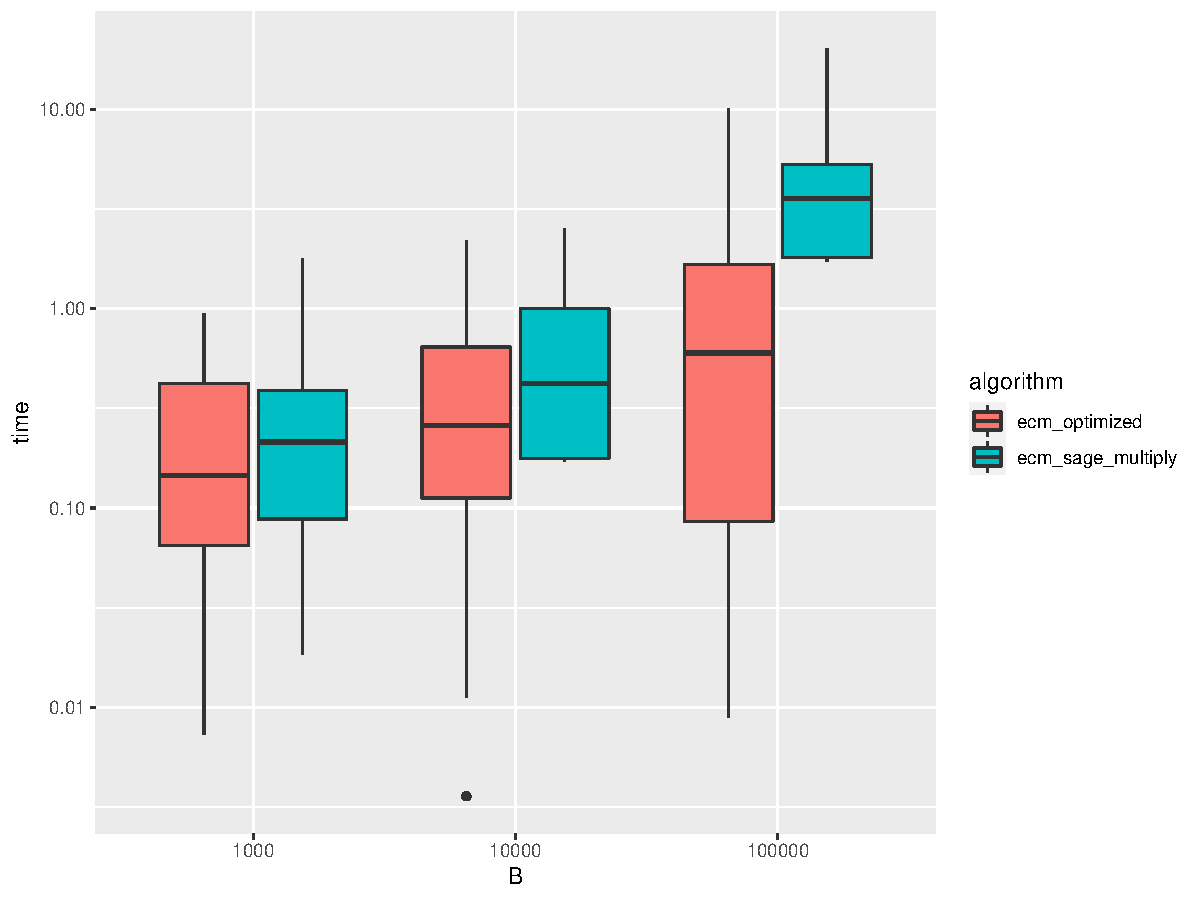
\includegraphics[width=\textwidth]{graphs/ecm_perf.pdf}

\end{frame}

\begin{frame}
\frametitle{Coded Example}

\lstinputlisting[language=Python]{ecm.sage}

\end{frame}

\begin{frame}
\frametitle{Animation 1 min}

\end{frame}

\end{document}
